\documentclass{article}
\usepackage{tikz}
\usetikzlibrary{lindenmayersystems}

\begin{document}
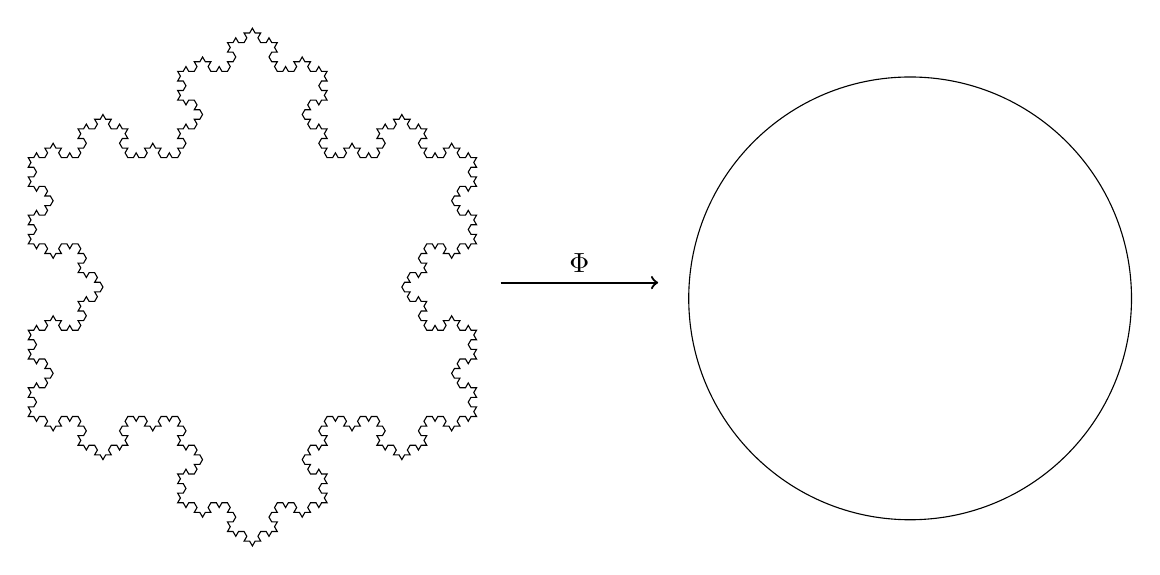
\begin{tikzpicture}
    \pgfdeclarelindenmayersystem{Koch curve}{
        \rule{F -> F-F++F-F}
        }
        \draw [black]
    [l-system={Koch curve, step=2pt, angle=60, axiom=F++F++F, order=4}]
    lindenmayer system -- cycle;

    \pgfmathsetmacro{\kochwidth}{2pt*4*10}
    \draw [black] (11.2,1.5) circle (\kochwidth pt);

    \draw [->, thick] (6,1.7) -- (8,1.7) node [midway, above] {$\Phi$};
\end{tikzpicture}


\end{document}